\def\ccTagRmEigenClassName{\ccFalse}
\def\ccLongParamLayout{\ccTrue}

\ccSetThreeColumns{Oriented_side}{}{\hspace*{10cm}}
\ccThreeToTwo

\chapter{dD Search Structures} 
\label{Trees}

%\ccChapterSubTitle{\rangetreeRevision, \rangetreeDate}

%\minitoc

\section{Introduction}

This chapter presents the {\cgal} range tree and segment tree
data structures. 

% The range tree is theoretically superior to the $Kd$-tree, but the 
% latter often seems to perform better.
% However, the range tree as implemented in {\cgal} is more flexible than the
% $Kd$-tree implementation, in that it enables to layer together range trees 
% and segment trees in the same data structure.

\section{Definitions}
This section presents $d$-dimensional range and segment trees.
A one-dimensional range tree is a binary search tree on 
{\em{one-dimensional point data}}. 
Here we call all one-dimensional data types having a strict ordering
(like integer and double) {\em point data}. 
{\em{$d$-dimensional point data}} are $d$-tuples of one-dimensional 
point data.

A one-dimensional segment tree is a binary search tree as well, but with
{\em{one-dimensional interval data}} as input data.
One-dimensional interval data is a pair (i.e., 2-tuple) $(a,b)$, where $a$ 
and $b$ are one-dimensional point data of the same type and $a< b$. 
The pair $(a,b)$ represents a half open interval $[a,b)$.
Analogously, a $d$-dimensional interval  is represented by a $d$-tuple of
one-dimensional intervals.

The {\em{input data type}} for a $d$-dimensional tree is a container 
class consisting of a $d$-dimensional point data type, interval data type 
or a mixture of both, and optionally a {\em{value type}}, which 
can be used to store arbitrary data. 
E.g., the $d$--dimensional bounding box of a $d$--dimensional polygon 
may define the interval data of a $d$--dimensional segment tree and
the polygon itself can be stored as its value.   
An {\em{input data item}} is an instance of an input data type.

The range and segment tree classes are fully generic in the sense that they 
can be used to define {\em{multilayer trees}}. 
A multilayer tree of dimension (number of layers) $d$ is a simple tree in 
the $d$-th layer, whereas the $k$-th layer, $1\leq k\leq d-1$, of the tree 
defines a tree where each (inner) vertex contains a multilayer tree of 
dimension $d-k+1$.
The $k-1$-dimensional tree which is nested in the $k$-dimensional tree 
($T$) is called the {\em sublayer tree} (of $T$).
For example, a $d$-dim tree can be a range tree on the first layer, 
constructed with respect to the first dimension of $d$-dimensional data 
items.
On all the data items in each subtree, a $(d-1)$-dimensional tree is built,
either a range or a segment tree, with respect to the second dimension of 
the data items.
And so on.
%E.g., for each inner vertex of a range tree, a sublayer tree is created 
%according to all data items of the subtree of that vertex. 
%For each vertex of a segment tree an instance (tree)  is created according 
%to all data items of that vertex.
%E.g., one can define a segment tree for which each vertex contains a 
%range tree.
\lcTex{
Figures~\ref{User:fig:range.eps}, \ref{User:fig:d-range.eps} and
\ref{User:fig:d-segment.eps} illustrate the meaning of a sublayer tree
graphically.
}
\lcHtml{
The figures in Sections~\ref{sec:range_trees} and~\ref{sec:segment_trees}
illustrate the means of a sublayer tree graphically.
}

After creation of the tree, further insertions or deletions of data items 
are disallowed.  
The tree class does neither depend on the type of data nor on the concrete
physical representation of the data items.
E.g., let a multilayer tree be a segment tree for which each vertex
defines a range tree. 
We can choose the data items to consist of intervals of type \ccStyle{double} 
and the point data of type \ccStyle{integer}. 
As value type we can choose  \ccStyle{string}.

For this generality we have to
define what the tree of each dimension looks like and how the
input data is organized.
For dimension $k$, $1\le k\le 4$, \cgal\/ provides ready-to-use
range and segment trees that can store k-dimensional keys
(intervals resp.). 
Examples illustrating the use of these classes are given in
Sections~\ref{sec:range_tree_ex}
and~\ref{sec:segment_tree_ex}.
The description of the functionality of these classes as well as
the definition of higher dimensional trees and mixed multilayer
trees is given in the reference manual.

In the following two sections we give short definitions of the version of
the range tree and segment tree implemented here together with some
examples. The presentation closely follows~\cite{bkos-cgaa-97}.

\section{Software Design}


\section{Range Trees}
A one-dimensional range tree is a binary search tree on one-dimensional 
point data. 
The point data of the tree is stored in the leaves. 
Each inner vertex stores the highest entry of its left subtree.
The version of a range tree implemented here is static, which means that 
after construction of the tree, no elements be inserted or deleted.
A $d$-dimensional range tree is a binary leaf search tree according to the 
first dimension of the $d$-dimensional point data, where each vertex contains 
a $(d-1)$-dimensional search tree of the points in the subtree (sublayer tree)
with respect to the second dimension.
See~\cite{bkos-cgaa-97} and~\cite{s-dasds-90} for more detailed information.

A $d$-dimensional range tree can be used to determine all
$d$-dimensional points that lie inside  a given $d$-dimensional
interval (\ccStyle{window\_query}).
\begin{ccTexOnly}
Figure~\ref{User:fig:range.eps} shows a two-dimensional range tree,
Figure~\ref{User:fig:d-range.eps} a $d$-dimensional one.
\end{ccTexOnly}
\begin{ccHtmlOnly}
The pictures below show a two-dimensional and a <MATH>d</MATH>-dimensional
range tree.
\end{ccHtmlOnly}
\begin{ccTexOnly}
    \begin{figure}[htbp]
    \begin{minipage}{7cm}
    \begin{center}
    \includegraphics[width=7cm,clip]{SearchStructures/range2.eps}
    \end{center}
    \caption{\label{User:fig:range.eps}A two-dimensional range tree. The
      tree is a binary search tree on the first dimension. Each
      sublayer tree of a vertex $v$ is a binary search tree on the second
      dimension. The data items in a sublayer tree of $v$ are
      all data items of the subtree of $v$.}
    \end{minipage}
    \hspace*{1em}
    \begin{minipage}{7cm}
    \begin{center}
    \includegraphics[width=7cm,clip]{SearchStructures/d-range.eps}
    \end{center}
    \caption{\label{User:fig:d-range.eps}A d-dimensional range tree. For
      each layer of the tree, one
      sublayer tree is illustrated.}
    \vspace{2\baselineskip}
    %
    \end{minipage}
    \end{figure}
\end{ccTexOnly}

\begin{ccHtmlOnly}
    <!2><TABLE BORDER=0 CELLSPACING=2 CELLPADDING=0 WIDTH=650>
        <TR><TD ALIGN=LEFT VALIGN=TOP WIDTH=50% NOWRAP COLSPAN=2>
    <A NAME="User:fig:range.eps"><img border=0 src="./range2.gif" alt="A two-dimensional range tree"></A>
    </TD>
    <A NAME="User:fig:d-range.eps"><TD ALIGN=LEFT VALIGN=TOP WIDTH=50%><img border=0 src="./d-range.gif" alt="A d-dimensional range tree"></A>
      </TD></TR></TABLE>
        <!2><TABLE BORDER=0 CELLSPACING=2 CELLPADDING=0 WIDTH=650>
        <TR><TD ALIGN=LEFT VALIGN=TOP WIDTH=45%  COLSPAN=2>
    A two-dimensional range tree. The
      tree is a binary search tree on the first dimension. Each
      sublayer tree of a vertex <MATH>v</MATH> is a binary search tree on the
second
      dimension. The data items in a sublayer tree of <MATH>v</MATH> are
      all data items of the subtree of <MATH>v</MATH>
 </TD><TD ALIGN=LEFT VALIGN=TOP WIDTH=50%>
A d-dimensional range tree. For
      each layer of the tree, one
      sublayer tree is illustrated.
 </TD></TR>
        </TABLE><!2>

\end{ccHtmlOnly}

%The tree can be built in  ${\cal O}(n\log^{d-1} n)$ time and
%needs  ${\cal O}(n\log^{d-1} n)$ space. The $d$-dimensional points that lie in the
%$d$-dimensional query interval can be reported in ${\cal O}(\log^dn+k)$ time,
%where $n$ is the total number of points and $k$ is the number of
%reported points. 

The tree can be built in  $O(n\log^{d-1} n)$ time and
needs  $O(n\log^{d-1} n)$ space. The $d$-dimensional points that lie in the
$d$-dimensional query interval can be reported in $O(\log^dn+k)$ time,
where $n$ is the total number of points and $k$ is the number of
reported points. 

\subsection{Example for Range Tree on Map-like Data\label{sec:range_tree_ex}}

The following example program uses the predefined \ccc{
  Range_tree_2} data structure together with the predefined traits
  class \ccc{Range_tree_map_traits_2} which has two template
  arguments specifying the
  type of the point data in each dimension
  (\ccc{CGAL::Cartesian<double>}) and the value type of the
  2-dimensional point data (\ccc{char}). Therefore the \ccc{
  Range_tree_2} is defined on 2-dimensional point data each of which is
  associated with a character.
Then, a few data items are created and put into a list. After
  that the tree is constructed according to that list, a window
  query is performed, and the query elements are given out.

\begin{verbatim}

#include <CGAL/Cartesian.h>
#include <CGAL/Range_segment_tree_traits.h>
#include <CGAL/Range_tree_k.h>

typedef CGAL::Cartesian<double> K;
typedef CGAL::Range_tree_map_traits_2<K, char> Traits;
typedef CGAL::Range_tree_2<Traits> Range_tree_2_type;

int main()
{
  typedef Traits::Key Key;                
  typedef Traits::Interval Interval;    

  std::vector<Key> InputList, OutputList;
  InputList.push_back(Key(K::Point_2(8,5.1), 'a'));
  InputList.push_back(Key(K::Point_2(1,1.1), 'b'));
  InputList.push_back(Key(K::Point_2(3,2.1), 'c'));

  Range_tree_2_type Range_tree_2(InputList.begin(),InputList.end());
  Interval win(Interval(K::Point_2(4,8.1),K::Point_2(5,8.2)));
  std::cout << "\n Window Query:\n ";
  Range_tree_2.window_query(win, std::back_inserter(OutputList));
  std::vector<Key>::iterator current=OutputList.begin();
  while(current!=OutputList.end()){
    std::cout << (*current).first.x() << "," << (*current).first.y()
         << ":" << (*current++).second << std::endl;
  }
}
\end{verbatim}



\subsection{Example for Range Tree on Set-like Data}

This example illustrates the use of the range tree on
2-dimensional point data (no value is associated to a data item).
After the definition of the tree, some input data items are
created and the tree is constructed according to the input data
items.
After that, a window query is performed and the query elements
are given to standard out.

\begin{verbatim}
#include <CGAL/Cartesian.h>
#include <CGAL/Range_segment_tree_traits.h>
#include <CGAL/Range_tree_k.h>

typedef CGAL::Cartesian<double> K;
typedef CGAL::Range_segment_tree_set_traits_2<K> Traits;
typedef CGAL::Range_tree_2<Traits> Range_tree_2_type;

int main()
{
  typedef Traits::Key Key;
  typedef Traits::Interval Interval;
  std::vector<Key> InputList, OutputList;
  std::vector<Key>::iterator first, last, current;

  InputList.push_back(Key(8,5.1));
  InputList.push_back(Key(1,1.1));
  InputList.push_back(Key(3,2.1));

  Range_tree_2_type Range_tree_2(InputList.begin(),InputList.end());

  Interval win=Interval(Key(4,8.1),Key(5,8.2));
  std::cout << std::endl << "Window Query: lower left point: (4.0,5.0),";
  std::cout << "upper right point: (8.1,8.2)" << std::endl;
  Range_tree_2.window_query(win, std::back_inserter(OutputList));
  current=OutputList.begin();
  while(current!=OutputList.end()){
    std::cout << (*current).x()<< "-" << (*current).y() << std::endl;
    current++;
  }
}
\end{verbatim}



\section{Segment Trees}
%\definition
A segment tree is a static binary search tree for a given set of
coordinates. The set of coordinates is defined by the endpoints
of the input data intervals. Any two adjacent coordinates
build an elementary interval. Every leaf corresponds to an
elementary interval.
Inner vertices
correspond to the union of the subtree intervals of the vertex.
Each vertex or leaf $v$ contains a sublayer type (or a
list, if it is one-dimensional) that will contain all intervals $I$, such that
$I$  contains the interval of vertex $v$ but not the interval
of the parent vertex of $v$.

A $d$-dimensional segment tree can be used to solve the following problems:
\begin{itemize}
\item Determine all $d$-dimensional intervals that contain a
  $d$-dimensional point. This query type is called ``inverse
  range query''.
  \item Determine all $d$-dimensional intervals that enclose a
    given $d$-dimensional interval
    (\ccStyle{enclosing\_query}).
  \item Determine all $d$-dimensional intervals that partially overlap or are
    contained in a given $d$-dimensional interval (\ccStyle{window\_query}).
\end{itemize}

\begin{ccTexOnly}
In Figure~\ref{User:fig:segment2.eps} an example of a one-dimensional segment 
tree is given. Figure~\ref{User:fig:d-segment.eps} shows a two-dimensional
segment tree.
\end{ccTexOnly}

\begin{ccHtmlOnly}
An example of a one-dimensional segment tree and an example
of a two-dimensional segment tree are shown below.
\end{ccHtmlOnly}

\begin{ccTexOnly}
\begin{figure}[htbp]
\centering
\begin{minipage}{11cm}
    \begin{center}
    \includegraphics[width=8cm,clip]{SearchStructures/segment2.eps}
    \end{center}
\caption{\label{User:fig:segment2.eps}A one-dimensional segment
  tree. The segments and the corresponding elementary intervals
  are shown below the tree. The arcs from the nodes point to
  their subsets.}
\vspace{2\baselineskip}
\end{minipage}
\hspace*{1em}
\begin{minipage}{11cm}
    \begin{center}
    \includegraphics[width=8cm,clip]{SearchStructures/d-segment.eps}
    \end{center}
\caption{\label{User:fig:d-segment.eps}A two-dimensional segment
  tree. The first layer of the tree is built according to the
  elementary intervals of the first dimension. Each
  sublayer tree of a vertex $v$ is a segment tree according to
  the  second dimension of all data items of $v$.}

\end{minipage}
\end{figure}
\end{ccTexOnly}

\begin{ccHtmlOnly}
    <!2><TABLE BORDER=0 CELLSPACING=2 CELLPADDING=0 WIDTH=650>
        <TR>
    <A NAME="User:fig:segment2.eps"></A>
    <TD ALIGN=LEFT VALIGN=TOP WIDTH=50% NOWRAP COLSPAN=2>
    <img border=0 src="./segment2.gif" alt="A one-dimensional segment
tree">
    </TD>
    <A NAME="User:fig:d-segment.eps"></A>
    <TD ALIGN=LEFT VALIGN=TOP WIDTH=50%><img border=0
src="./d-segment.gif" alt="A d-dimensional segment tree">
      </TD></TR></TABLE>

        <!2><TABLE BORDER=0 CELLSPACING=2 CELLPADDING=0 WIDTH=650>
        <TR><TD ALIGN=LEFT VALIGN=TOP WIDTH=50%  COLSPAN=2>
A one-dimensional segment
  tree. The segments and the corresponding elementary intervals
  are shown below the tree. The arcs from the nodes point to
  their subsets.
 </TD><TD ALIGN=LEFT VALIGN=TOP WIDTH=45%>
A two-dimensional segment
  tree. The first layer of the tree is built according to the
  elementary intervals of the first dimension. Each
  sublayer tree of a vertex  <MATH>v</MATH> is a segment tree according to
  the  second dimension of all data items of  <MATH>v</MATH>.
 </TD></TR>
        </TABLE><!2>
\end{ccHtmlOnly}

%The tree can be built in  ${\cal O}(n\log^{d} n)$ time and
%needs  ${\cal O}(n\log^{d} n)$ space.
%The  processing time for inverse range
%queries in an $d$-dimensional segment tree is ${\cal O}(\log^d n
%+k)$ time, where $n$ is the total number of intervals and $k$ is
%the number of reported intervals.
The tree can be built in  $O(n\log^{d} n)$ time and
needs  $O(n\log^{d} n)$ space.
The  processing time for inverse range
queries in an $d$-dimensional segment tree is $O(\log^d n
+k)$ time, where $n$ is the total number of intervals and $k$ is
the number of reported intervals.

One possible application of a two-dimensional segment tree is the
following. Given a set of convex polygons in two-dimensional
space (CGAL::Polygon\_2), we want to determine all polygons
that intersect a given rectangular query window. Therefore, we define a
two-dimensional segment tree, where the two-dimensional interval of
a data item corresponds to the  bounding box of a polygon and the
value type corresponds to the polygon itself. The segment tree is created
with a sequence of all data items, and a window query is
performed. The polygons of the resulting data items are finally
tested independently for intersections.



\subsection{Example for Segment Tree on Map-like Data\label{sec:segment_tree_ex}}

The following example program uses the predefined \ccc{
  Segment_tree_2} data structure together with the predefined traits
  class \ccc{Segment_tree_map_traits_2} which has two template arguments
  specifying the
  type of the point data in each dimension
  (\ccc{CGAL::Cartesian<double>}) and the value type of the
  2-dimensional point data (\ccc{char}). Therefore the \ccc{
  Segment_tree_2} is defined on 2-dimensional point data
  (\ccc{CGAL::Point_2<Cartesian<double> >}) each of which is
  associated with a character.
Then, a few data items are created and put into a list. After
  that the tree is constructed according to that list, a window
  query is performed, and the query elements are given out.



\begin{verbatim}
#include <CGAL/Cartesian.h>
#include <CGAL/Segment_tree_k.h>
#include <CGAL/Range_segment_tree_traits.h>

typedef CGAL::Cartesian<double> K;
typedef CGAL::Segment_tree_map_traits_2<K, char> Traits;
typedef CGAL::Segment_tree_2<Traits > Segment_tree_2_type;

int main()
{
  typedef Traits::Interval Interval;
  typedef Traits::Pure_interval Pure_interval;
  typedef Traits::Key Key;
  std::list<Interval> InputList, OutputList1, OutputList2;

  InputList.push_back(Interval(Pure_interval(Key(1,5), Key(2,7)),'a'));
  InputList.push_back(Interval(Pure_interval(Key(2,7), Key(3,8)),'b'));
  InputList.push_back(Interval(Pure_interval(Key(6,9), Key(9,13)),'c'));
  InputList.push_back(Interval(Pure_interval(Key(1,3), Key(3,9)),'d'));
 
  Segment_tree_2_type Segment_tree_2(InputList.begin(),InputList.end());

  Interval a=Interval(Pure_interval(Key(3,6), Key(7,12)),'e');
  Segment_tree_2.window_query(a,std::back_inserter(OutputList1));

  std::list<Interval>::iterator j = OutputList1.begin();
  std::cout << "\n window_query (3,6),(7,12)\n";
  while(j!=OutputList1.end()){
    std::cout << (*j).first.first.x() << "-" << (*j).first.second.x() << " " 
         << (*j).first.first.y() << "-" << (*j).first.second.y() << std::endl; 
    j++;
  }
  
  Interval b=Interval(Pure_interval(Key(6,10),Key(7,11)), 'f');
  Segment_tree_2.enclosing_query(b,std::back_inserter(OutputList2));
  j = OutputList2.begin();
  std::cout << "\n enclosing_query (6,10),(7,11)\n";
  while(j!=OutputList2.end()){
    std::cout << (*j).first.first.x() << "-" << (*j).first.second.x() << " " 
         << (*j).first.first.y() << "-" << (*j).first.second.y() << std::endl; 
    j++;
  }
  return 0; 
}

\end{verbatim}

\subsection{Example for Segment Tree on Set-like Data}

This example illustrates the use of the predefined segment tree
on 3-dimensional interval data (with no value associated). After
the definition of the traits type and tree type, some intervals
are constructed and the tree is build according to the
intervals. Then, a window query is performed and the query
elements are given out.

\begin{verbatim}
#include <CGAL/Cartesian.h>
#include <CGAL/Segment_tree_k.h>
#include <CGAL/Range_segment_tree_traits.h>

typedef CGAL::Cartesian<int> K;
typedef CGAL::Range_segment_tree_set_traits_3<K> Traits;
typedef CGAL::Segment_tree_3<Traits > Segment_tree_3_type;

int main()
{
  typedef Traits::Interval Interval;
  typedef Traits::Key Key;
  std::list<Interval> InputList, OutputList;

  InputList.push_back(Interval(Key(1,5,7), Key(2,7,9)));
  InputList.push_back(Interval(Key(2,7,6), Key(3,8,9)));
  InputList.push_back(Interval(Key(6,9,5), Key(9,13,8)));
  InputList.push_back(Interval(Key(1,3,4), Key(3,9,8)));
 
  Segment_tree_3_type Segment_tree_3(InputList.begin(),InputList.end());

  Interval a(Key(3,6,5), Key(7,12,8));
  Segment_tree_3.window_query(a,std::back_inserter(OutputList));
  std::list<Interval>::iterator j = OutputList1.begin();
  std::cout << "\n window_query (3,6,5),(7,12,8) \n";
  while(j!=OutputList.end()){
    std::cout << (*j).first.x() << "," << (*j).first.y() << ",";
    std::cout << (*j).first.z() <<", " << (*j).second.x() << ",";
    std::cout << (*j).second.y() << "," << (*j).second.z() << std::endl; 
    j++;
  }
}
\end{verbatim}



\section{Interval Skip List}


% +========================================================================+
\subsection{Definition}
% +========================================================================+
  
An interval skip list is a data strucure for finding all intervals 
that contain a point, and for stabbing queries, that is for answering 
the question whether a given point is contained in an interval or not. 
The implementation we provide is dynamic, that is the user can freely
mix calls  to the methods \ccc{insert(..)}, \ccc{remove(..)}, 
\ccc{find_intervals(..)}, and \ccc{is_contained(..)}

The interval skip list class is parameterized with an interval class.

The data structure was introduced by Hanson~\cite{}, and it is called
interval skip list, because it is an extension of the randomized list
structure known as skip list~\cite{}. .
 
% +========================================================================+
\subsection{Example Programs}
% +========================================================================+
\label{sectionIntervalskiplistExamples}

We give two examples. The first one uses a basic interval class.  In
the second example we create an interval skip list for the $z$-ranges
of the faces of a terrain, allowing to answer level queries.

% +-------------------------------------------------------------+
\subsubsection{First Example with Simple Interval}

The first example reads two numbers \ccc{n} and \ccc{d} from \ccc{std::cin}.
It creates n intervals of length \ccc{d} with the left endpoint at \ccc{n}.
It then reads out the intervals for the 1-dimensional points with
coordinates $0 ... n+d$. 

The interval skip list class has as template argument an interval
class. In this example we use the class \ccc{Interval_skip_list_interval}.

\newpage
\ccIncludeExampleCode{Interval_skip_list/intervals.C}

% +-------------------------------------------------------------+
\subsubsection{Example with Faces of a Triangulated Terrain}



This example creates an interval skip list that allows to find all the faces
of a terrain intersected by an horizontal plane with given level.
The data points for the terain are  read from a file. 

As model for the interval concept, we use a class that is a wrapper
around a face handle of a triangulated terrain. Lower and upper bound
of the interval are smallest and largest $z$-coordinate of the face.

\ccIncludeExampleCode{Interval_skip_list/terrain.C}


% +--------------------------------------------------------+

%% =============================================================================
% The CGAL Reference Manual
% Chapter: Optimisation
% -----------------------------------------------------------------------------
% file  : doc_tex/basic/Optimisation/main.tex
% author: Bernd G�rtner, Sven Sch�nherr (sven@inf.fu-berlin.de)
% -----------------------------------------------------------------------------
% $Revision$
% $Date$
% =============================================================================

\newcommand{\linebreakByHand}{\ccTexHtml{\\}{}}
\newcommand{\SaveSpaceByHand}{}  %%%% [2]{\ccTexHtml{#1}{#2}}

\chapter{Geometric Optimisation} \label{Optimisation}
\RCSdefDate{\OptRCSDate}{$Date$}

\ccChapterRelease{Release: 2.0 \ccTexHtml{\quad}{ , } \OptRCSDate}

\ccChapterAuthor{Bernd G{\"a}rtner}\ccTexHtml{\\}{<br>}
\ccChapterAuthor{Michael Hoffmann}\ccTexHtml{\\}{<br>}
\ccChapterAuthor{Sven Sch{\"o}nherr}

\ccTexHtml{\thispagestyle{empty}}{}

\begin{ccTexOnly}\section*{Introduction}\end{ccTexOnly}
\begin{ccHtmlOnly}<H2>Introduction</H2><P>\end{ccHtmlOnly}

This chapter describes routines for solving geometric optimisation problems.
The first two sections contain algorithms for computing and updating the
smallest enclosing circle (Section~\ref{sec:smallest_enclosing_circles})
resp.\ ellipse (Section~\ref{sec:smallest_enclosing_ellipses}) of a finite
point set.  Formally, the `smallest enclosing circle' is the boundary of the
closed disk of minimum area covering the point set. It is known that this
disk is unique.  We usually identify the disk with its bounding circle,
allowing us to talk about points being on the boundary of the circle, etc.
The same holds for the smallest enclosing ellipse. These algorithms work in
an incremental manner. They are implemented as semi-dynamic data structures,
thus allowing to insert points while maintaining the smallest enclosing
circle resp.\ ellipse.

The remaining sections describe algorithms for searching in matrices with
specific properties and some applications. In particular, there are
general implementations of
\begin{itemize}
  \item monotone matrix search (see Section~\ref{secMonotoneMatrixSearch}),
    which can be applied to compute
    \begin{itemize}
      \item extremal polygons of a convex polygon
        (see Section~\ref{secComputingExtremalPolygons}) \textit{or}
      \item all furthest neighbors for the vertices of a convex polygon
        (see Section~\ref{secAllFurthestNeighbors}),
    \end{itemize}
  \item and sorted matrix search (see Section~\ref{secSortedMatrixSearch}),
    which can be used to compute the $p$-centers of a planar point set
    (see Section~\ref{sec_RectangularPCenters}).
\end{itemize}

\subsubsection*{Traits Class}
The class and function templates are parameterized with a traits class
which defines the abstract interface between the optimisation
algorithm and the primitives it uses. We provide traits class
implementations that interface the optimisation algorithms with the
\cgal\ kernel. For some algorithms, in addition, we provide traits
class adapters to user supplied point classes. Finally, we describe
the requirements that must be fulfilled by traits classes for
optimisation algorithms.  This is at the same time a specification for
using the provided traits class implementations as for users who want
to supply their own traits class.

\subsubsection*{Assertions}
The optimisation code uses infix \ccc{OPTIMISATION} in the assertions,
e.g.\ defining the compiler flag
\ccc{CGAL_OPTIMISATION_NO_PRECONDITIONS} switches precondition
checking off, cf.~Section~\ref{assertions}.

\newcommand{\cgalSetOptTraitsAdaptLayout}{\ccTexHtml{%
    \ccSetThreeColumns{CGAL_Oriented_side}{}{returns constants
      \ccc{CGAL_LEFTTURN}, \ccc{CGAL_COLLINEAR}}
    \ccPropagateThreeToTwoColumns}{}}
\newcommand{\cgalSetOptTraitsAdaptReqLayout}{\ccTexHtml{%
    \ccSetThreeColumns{CGAL_Oriented_side}{da.get_hw( Point p).}{}
    \ccPropagateThreeToTwoColumns}{}}

\newcommand{\cgalSetOptTraitsReqLayout}{\ccTexHtml{%
    \ccSetThreeColumns{CGAL_Oriented_side}{}{returns
      \ccc{CGAL_ON_BOUNDED_SIDE}, \ccc{CGAL_ON_BOUNDARY}}
    \ccPropagateThreeToTwoColumns}{}}

\ccHtmlNoClassToc

\input{smallest_enclosing_circles}

\input{smallest_enclosing_ellipses}

%% ==============================================================
%% Specification: Computing Extremal Polygons
%% --------------------------------------------------------------
%% file  : spec_extremal_polygons.awi
%% author: Michael Hoffmann
%% $Id$
%% ==============================================================

\clearpage
\section{Computing Extremal Polygons}
\label{secComputingExtremalPolygons}
\cgalColumnLayout

This section describes several functions to compute a maximal $k$-gon
$P_k$ that can be inscribed into a given convex polygon $P$. The
criterion for maximality can be chosen freely by defining an
appropriate traits class as specified in section
\ref{req_ExtremalPolygonTraits}. For \cgal\ point classes there are
two predefined traits classes to compute a maximum area (see section
\ref{secMaximumAreaInscribedKgon}) resp.  perimeter (see section
\ref{secMaximumPerimeterInscribedKgon}) inscribed $k$-gon.

\ccHtmlNoClassToc
\begin{ccHtmlClassFile}{computing_maximum_area_inscribed_k_gon.html}
  {Function Declaration of \ccc{maximum_area_inscribed_k_gon}}
  \ccHtmlNoClassIndex\ccHtmlNoClassLinks
  %% class wrapper to keep the font at a uniform size:
  \begin{ccClass}{dummy}
    \ccHtmlNoIndex\subsection{Computing a Maximum Area Inscribed $k$-gon}
  \label{secMaximumAreaInscribedKgon}
  \end{ccClass}
  
  This section describes a function to compute a maximal area $k$-gon
  $P_k$ that can be inscribed into a given convex polygon $P$. Note
  that $P_k$ is not unique in general, but it can be chosen in such a
  way that its vertices form a subset of the vertex set of $P$.

  \ccInclude{CGAL/extremal_polygon_2.h}

  \def\ccLongParamLayout{\ccTrue} 
  
  \ccGlobalFunction{
    template < class RandomAccessIC, class OutputIterator >
    OutputIterator
    maximum_area_inscribed_k_gon(
    RandomAccessIC points_begin,
    RandomAccessIC points_end,
    int k,
    OutputIterator o);}
  
  computes a maximum area inscribed $k$-gon of the convex polygon
  described by [\ccc{points_begin}, \ccc{points_end}), writes its
  vertices to \ccc{o} and returns the past-the-end iterator of this
  sequence.
  
  \ccHeading{Precondition}
  \begin{enumerate}
  \item Value type of \ccc{RandomAccessIC} has to be
    \ccc{Point_2<R>} for some representation class \ccc{R}.
  \item \ccc{OutputIterator} accepts the value type of
    \ccc{RandomAccessIC} as value type,
  \item the -- at least three -- points denoted by the range
    [\ccc{points_begin}, \ccc{points_end}) form the boundary of a convex
    polygon (oriented clock-- or counterclockwise) \textit{and}
  \item $k \ge 3$.
  \end{enumerate}

  \ccHeading{Note}
  
  On compilers not supporting member function templates, the parameter
  \ccc{RandomAccessIC} is fixed to \ccc{vector<Point_2>::iterator}
  where \ccc{Point_2} is the value type of \ccc{RandomAccessIC}.
  
  \ccImplementation The implementation uses monotone matrix
  search\cite{akmsw-gamsa-87} and has a worst case running time of $O(k
  \cdot n + n \cdot \log n)$, where $n$ is the number of vertices in
  $P$.

  \ccExample The following code generates a random convex polygon
  \ccc{p} with ten vertices and computes the maximum area inscribed
  five-gon of \ccc{p}.

  \ccIncludeVerbatim{extremal_polygon_2_example_area.C}

\end{ccHtmlClassFile}
    
\ccHtmlNoClassToc
\begin{ccHtmlClassFile}{computing_maximum_perimeter_inscribed_k_gon.html}
  {Function Declaration of \ccc{maximum_perimeter_inscribed_k_gon}}
  \ccHtmlNoClassIndex\ccHtmlNoClassLinks
  %% class wrapper to keep the font at a uniform size:
  \begin{ccClass}{dummy}
    \ccHtmlNoIndex\subsection{Computing a Maximum Perimeter Inscribed
      $k$-gon}
    \label{secMaximumPerimeterInscribedKgon}
  \end{ccClass}
  
  This section describes a function to compute a largest perimeter
  $k$-gon $P_k$ that can be inscribed in a given convex polygon $P$.
  Note that $P_k$ is not unique in general, but we know that its
  vertices form a subset of the vertex set of $P$.

  \ccInclude{CGAL/extremal_polygon_2.h}

  \def\ccLongParamLayout{\ccTrue}
  \ccGlobalFunction{
    template < class RandomAccessIC, class OutputIterator >
    OutputIterator
    maximum_perimeter_inscribed_k_gon(
    RandomAccessIC points_begin,
    RandomAccessIC points_end,
    int k,
    OutputIterator o);}
  
  computes a maximum perimeter inscribed $k$-gon of the convex polygon
  described by [\ccc{points_begin}, \ccc{points_end}), writes its
  vertices to \ccc{o} and returns the past-the-end iterator of this
  sequence.

  \ccHeading{Precondition}
  \begin{enumerate}
  \item Value type of \ccc{RandomAccessIC} has to be
    \ccc{Point_2<R>} for some representation class \ccc{R},
  \item there is a global function \ccc{R::FT sqrt( R::FT)}
    defined that computes the squareroot of a number,
  \item \ccc{OutputIterator} accepts the value type of
    \ccc{RandomAccessIC} as value type,
  \item the -- at least three -- points denoted by the range
    [\ccc{points_begin}, \ccc{points_end}) form the boundary of a
    convex polygon (oriented clock-- or counterclockwise) \textit{and}
  \item $k \ge 2$.
  \end{enumerate}

  \ccTagDefaults

  \ccHeading{Note}
  
  On compilers not supporting member function templates, the parameter
  \ccc{RandomAccessIC} is fixed to \ccc{vector<Point_2>::iterator}
  where \ccc{Point_2} is the value type of \ccc{RandomAccessIC}.
  
  \ccImplementation The implementation uses monotone matrix
  search\cite{akmsw-gamsa-87} and has a worst case running time of $O(k
  \cdot n + n \cdot \log n)$, where $n$ is the number of vertices in
  $P$.

  \ccExample The following code generates a random convex polygon
  \ccc{p} with ten vertices and computes the maximum perimeter inscribed
  five-gon of \ccc{p}.

  \ccIncludeVerbatim{extremal_polygon_2_example_perimeter.C}

\end{ccHtmlClassFile}

\begin{ccAdvanced}
  \ccHtmlNoClassToc
  \begin{ccHtmlClassFile}{computing_general_extremal_polygons.html}
    {Function Declaration of \ccc{extremal_polygon}}
    \ccHtmlNoClassIndex\ccHtmlNoClassLinks
    %% class wrapper to keep the font at a uniform size:
    \begin{ccClass}{dummy}
      \ccHtmlNoIndex\subsection{Computing General Extremal
        Polygons}\label{secGeneralExtremalPolygons}
    \end{ccClass}
    
    This section describes a general function to compute a maximal
    $k$-gon $P_k$ that can be inscribed in a given convex polygon $P$.
    The criterion for maximality and some basic operations have to
    specified in an appropriate traits class as specified in section
    \ref{req_ExtremalPolygonTraits}.
    
    \ccInclude{CGAL/extremal_polygons_2.h}

    \def\ccLongParamLayout{\ccTrue} 
    
    \ccGlobalFunction{
      template < class RandomAccessIC, class OutputIterator, class Traits >
      OutputIterator
      extremal_polygon(
      RandomAccessIC points_begin,
      RandomAccessIC points_end,
      int k,
      OutputIterator o,
      const Traits& t);}
    
    computes a maximal (as specified by \ccc{t}) inscribed $k$-gon of
    the convex polygon described by [\ccc{points_begin},
    \ccc{points_end}), writes its vertices to \ccc{o} and returns the
    past-the-end iterator of this sequence.
    
    \ccHeading{Precondition}
    \begin{enumerate}
    \item \ccc{Traits} has to satisfy the requirements stated in section
      \ref{req_ExtremalPolygonTraits},
    \item Value type of \ccc{RandomAccessIC} must be
      \ccc{Traits::Point_2},
    \item \ccc{OutputIterator} accepts \ccc{Traits::Point_2} as value
      type,
    \item the -- at least three -- points denoted by the range
      [\ccc{points_begin}, \ccc{points_end}) form the boundary of a
      convex polygon (oriented clock-- or counterclockwise) \textit{and}
    \item $k \ge \ccc{t.min_k()}$.
    \end{enumerate}
    
    \ccImplementation The implementation uses monotone matrix
    search\cite{akmsw-gamsa-87} and has a worst case running time of
    $O(k \cdot n + n \cdot \log n)$, where $n$ is the number of vertices
    in $P$.
  \end{ccHtmlClassFile}
  
  \ccHtmlNoClassToc\ccHtmlNoClassIndex\begin{ccClass}{Exp_traits}
    \ccCreationVariable{t}\ccTagFullDeclarations
    
    \subsection{Requirements for Extremal Polygon Traits
      Classes}\label{req_ExtremalPolygonTraits}
    
    \ccDefinition A class \ccClassName\ has to provide the following
    types and operations in order to qualify as a traits class for
    \ccc{extremal_polygon}.
    
    \ccTypes 
    
    \ccNestedType{Point_2}{class used for representing the input
      points.}
    
    \ccNestedType{FT}{class used for doing computations on point
      coordinates (has to fulfill field-type requirements).}
    
    \ccNestedType{Operation}{AdaptableBinaryFunction class \ccc{op}:
      \ccc{Point_2} $\times$ \ccc{Point_2} $\rightarrow$ \ccc{FT}.
      Together with \ccc{init} this operation recursively defines the
      objective function to maximize.  Let $p$ and $q$ be two vertices
      of a polygon $P$ such that $q$ precedes $p$ in the oriented
      vertex chain of $P$ starting with vertex $root$.  Then
      \ccc{op(p,q)} returns the value by which an arbitrary
      sub-polygon of $P$ with vertices from $[root,\, q]$ increases
      when $p$ is added to it. E.g. in the maximum area case this is
      the area of the triangle $(root,\, q,\, p)$.}

    \ccOperations
    
    \ccMemberFunction{int min_k() const;}{returns the minimal $k$ for
      which a maximal $k$-gon can be computed. (e.g. in the maximum
      area case this is three.)}
    
    \ccMemberFunction{FT init( const Point_2& p, const Point_2& q)
      const;}{returns the value of the objective function for a
      polygon consisting of the two points \ccc{p} and \ccc{q}. (e.g.
      in the maximum area case this is \ccc{FT( 0)}.)}
    
    \ccMemberFunction{Operation operation( const Point_2& p)
      const;}{return \ccc{Operation} where \ccc{p} is the fixed $root$
      point.}
    
    \ccMemberFunction{template < class RandomAccessIC, class
      OutputIterator > OutputIterator compute_min_k_gon(
      RandomAccessIC points_begin, RandomAccessIC points_end, FT&
      max_area, OutputIterator o) const;}{writes the points of
      [\ccc{points_begin}, \ccc{points_end}) forming a
      \ccc{min_k()}-gon rooted at \ccc{points_begin[0]} of maximal
      value to o and returns the past-the-end iterator for that
      sequence (== \ccc{o + min_k()}).}
    
    \ccMemberFunction{template < class RandomAccessIC > bool
      is_convex( RandomAccessIC points_begin, RandomAccessIC
      points_end) const;}{returns true, iff the points
      [\ccc{points_begin}, \ccc{points_end}) form a convex chain.}
    
    \ccHeading{Notes}
    \begin{itemize}
    \item \ccClassName\ccc{::is_convex} is only used for precondition
      checking. Therefore it needs not to be specified, in case that
      precondition checking is disabled.
    \item On compilers not supporting member function templates,
      \ccc{RandomAccessIC} is fixed to \ccc{vector<Point_2>::iterator}
      and \ccc{OutputIterator} is fixed to
      \ccc{vector<int>::reverse_iterator}.
      
    \end{itemize}
    
    \ccSeeAlso \ccInclude{CGAL/Extremal_polygon_traits_2.h}
    
    The classes \ccc{Kgon_area_traits<R>} and
    \ccc{Kgon_perimeter_traits<R>} (templatized with a \cgal\ 
    representation class) both fulfill these requirements.
    
  \end{ccClass}
\end{ccAdvanced}

%% --------------------------------------------------------------
%% EOF spec_extremal_polygons.awi
%% --------------------------------------------------------------

 
%% ==============================================================
%% Specification: All Furthest Neighbors
%% --------------------------------------------------------------
%% file  : spec_all_furthest_neighbors.awi
%% author: Michael Hoffmann
%% $Id$
%% ==============================================================

\cgalColumnLayout

\begin{ccRefFunction}{all_furthest_neighbors_2}
  
  \ccDefinition The function \ccRefName\ computes all furthest
  neighbors for the vertices of a convex polygon $P$, i.e. for each
  vertex $v$ of $P$ a vertex $f_v$ of $P$ such that the distance
  between $v$ and $f_v$ is maximized.

  \ccInclude{CGAL/all_furthest_neighbors_2.h}

  \def\ccLongParamLayout{\ccTrue} 
  
  \ccGlobalFunction{ template < class RandomAccessIC, class
    OutputIterator, class Traits > OutputIterator
    all_furthest_neighbors_2( RandomAccessIC points_begin,
    RandomAccessIC points_end, OutputIterator o, Traits t =
    Default_traits);}
  
  computes all furthest neighbors for the vertices of the convex
  polygon described by the range [\ccc{points_begin},
  \ccc{points_end}), writes their indices (relative to
  \ccc{points_begin}) to \ccc{o}\footnote{i.e. the furthest neighbor
    of \ccc{points_begin[}i\ccc{]} is \ccc{points_begin[}$i$-th number
    written to \ccc{o}\ccc{]}} and returns the past-the-end iterator
  of this sequence.
  
  \ccPrecond The points denoted by the non-empty range
  [\ccc{points_begin}, \ccc{points_end}) form the boundary of a convex
  polygon $P$ (oriented clock-- or counterclockwise).
  
  The geometric types and operations to be used for the computation
  are specified by the traits class parameter \ccc{t}. This parameter
  can be omitted if \ccc{RandomAccessIC} refers to a point type from
  the 2D-Kernel. In this case, a default traits class
  (\ccc{All_furthest_neighbors_default_traits_2<R>}) is used.
  
  \ccRequire
  \begin{enumerate}
  \item If \ccc{t} is specified explicitly, \ccc{Traits} is a model
    for \ccc{All_furthest_neighbors_traits_2}.
  \item Value type of \ccc{RandomAccessIC} is \ccc{Traits::Point_2} or
    -- if \ccc{t} is not specified explicitly -- \ccc{Point_2<R>} for
    some representation class \ccc{R}.
  \item \ccc{OutputIterator} accepts \ccc{int} as value type.
  \end{enumerate}
  
  \ccSeeAlso
  \ccRefIdfierPage{All_furthest_neighbors_traits_2}\\
  \ccRefIdfierPage{CGAL::All_furthest_neighbors_default_traits_2<R>}\\
  \ccRefIdfierPage{CGAL::monotone_matrix_search}
 
  \ccImplementation The implementation uses monotone matrix
  search\cite{akmsw-gamsa-87}. Its runtime complexity is linear in the
  number of vertices of $P$.
  
  \ccExample The following code generates a random convex polygon
  \ccc{p} with ten vertices, computes all furthest neighbors and
  writes the sequence of their indices (relative to
  \ccc{points_begin}) to \ccc{cout} (e.g. a sequence of
  \ccc{4788911224} means the furthest neighbor of
  \ccc{points_begin[0]} is \ccc{points_begin[4]}, the furthest
  neighbor of \ccc{points_begin[1]} is \ccc{points_begin[7]} etc.).
  
  \ccIncludeVerbatim{Optimisation_ref/all_furthest_neighbors_2_example_noheader.C}
\end{ccRefFunction}

\begin{ccRefClass}{All_furthest_neighbors_default_traits_2<R>}
  \ccCreationVariable{t}\ccTagFullDeclarations
  
  \ccDefinition The class \ccClassName\ provides the types and
  operations needed to compute all furthest neighbors for the vertices
  of a convex polygon.
  
  \ccRequirements
  The template parameter \ccc{R} is a model for \ccc{Kernel}.

  \ccIsModel 
  \ccRefIdfierPage{All_furthest_neighbors_traits_2}

  \ccTypes
  
  \ccNestedType{Point_2}{typedef to \ccc{R::Point_2}.}
  
  \ccNestedType{FT}{typedef to \ccc{R::FT}.}
  
  \ccNestedType{Distance}{AdaptableBinaryFunction class: \ccc{Point_2}
    $\times$ \ccc{Point_2} $\rightarrow$ \ccc{FT} computing the
    squared Euclidean distance between two points.}

  \ccOperations
  
  \ccMemberFunction{Distance distance_object();}{returns the
    function object for computing distances.}
  
  \ccMemberFunction{template < class RandomAccessIC > bool is_convex(
    RandomAccessIC points_begin, RandomAccessIC points_end)
    const;}{returns true, iff the points [\ccc{points_begin},
    \ccc{points_end}) form a convex chain.}
  
  \ccSeeAlso
  \ccRefIdfierPage{CGAL::all_furthest_neighbors_2}

  \ccHeading{Notes}
  \begin{itemize}
  \item \ccClassName\ccc{::is_convex} is used for precondition
    checking only.
  \end{itemize}
\end{ccRefClass}

\begin{ccRefConcept}{All_furthest_neighbors_traits_2}
  \ccCreationVariable{t}\ccTagFullDeclarations
  
  \ccDefinition The concept \ccRefName\ defines types and operations
  needed to compute all furthest neighbors for the vertices of a
  convex polygon using the function \ccc{all_furthest_neighbors_2}.
  
  \ccTypes
  
  \ccNestedType{Point_2}{class used for representing the input
    points.}
  
  \ccNestedType{FT}{class used for doing computations on point
    coordinates; it has to be a model for \ccc{FieldNumberType}.}
  
  \ccNestedType{Distance}{AdaptableBinaryFunction class: \ccc{Point_2}
    $\times$ \ccc{Point_2} $\rightarrow$ \ccc{FT} computing the
    squared Euclidean distance between two points.}

  \ccOperations
  
  \ccMemberFunction{Distance distance_object();}{returns the
    function object for computing distances.}
  
  \ccMemberFunction{template < class RandomAccessIC > bool is_convex(
    RandomAccessIC points_begin, RandomAccessIC points_end)
    const;}{returns true, iff the points [\ccc{points_begin},
    \ccc{points_end}) form a convex chain.}
  
  \ccHasModels 
  \ccRefIdfierPage{CGAL::All_furthest_neighbors_default_traits_2<R>}

  \ccSeeAlso
  \ccRefIdfierPage{CGAL::all_furthest_neighbors_2}

  \ccHeading{Notes}
  \begin{itemize}
  \item \ccClassName\ccc{::is_convex} is used for precondition
    checking only.
  \end{itemize}
\end{ccRefConcept}

%% --------------------------------------------------------------
%% EOF spec_all_furthest_neighbors.awi
%% --------------------------------------------------------------

 
%% ==============================================================
%% Specification: Rectangular p-Centers
%% --------------------------------------------------------------
%% file  : spec_rectangular_p_centers.awi
%% author: Michael Hoffmann
%% $Id$
%% ==============================================================

\cgalColumnLayout

\begin{ccRefFunction}{rectangular_p_center_2}
  \ccIndexMainItem[t]{rectilinear centers}
  \ccIndexMainItem[t]{rectangular centers}
  \ccIndexSubitem[t]{center}{rectangular}
  
  \ccDefinition The function \ccRefName\ computes rectilinear
  $p$-centers of a planar point set, i.e. a set of $p$ points such
  that the maximum minimal $L_{\infty}$-distance between both sets is
  minimized.
  
  More formally the problem can be defined as follows.
  
  \ccTexHtml{Given a finite set $\mathcal{P}$ of points, compute a
    point set $\mathcal{C}$ with $|\mathcal{C}| \le p$ such that the
    $p$-radius of $\mathcal{P}$,
    $$
    rad_p(\mathcal{P}) := \max_{P \in \mathcal{P}} \min_{Q \in
      \mathcal{C}} || P - Q ||_\infty
    $$
    is minimized. We can interpret $\mathcal{C}$ as the best
    approximation (with respect to the given metric) for $\mathcal{P}$
    with at most $p$ points.}{Given a finite set <IMG WIDTH=12
    HEIGHT=12 ALIGN=BOTTOM ALT="tex2html_wrap_inline17"
    SRC="./MatrixSearch_pcenter1.gif" > of points, compute a point set
    <IMG WIDTH=9 HEIGHT=13 ALIGN=BOTTOM ALT="tex2html_wrap_inline19"
    SRC="./MatrixSearch_pcenter2.gif" > with <IMG WIDTH=46 HEIGHT=24
    ALIGN=MIDDLE ALT="tex2html_wrap_inline21"
    SRC="./MatrixSearch_pcenter3.gif" > such that the <I>p</I>-radius
    of <IMG WIDTH=12 HEIGHT=12 ALIGN=BOTTOM
    ALT="tex2html_wrap_inline17" SRC="./MatrixSearch_pcenter1.gif" > ,
    <P> <IMG WIDTH=358 HEIGHT=24 ALIGN=BOTTOM ALT="displaymath27"
    SRC="./MatrixSearch_pcenter4.gif" > <P> is minimized. We can
    interpret <IMG WIDTH=9 HEIGHT=13 ALIGN=BOTTOM
    ALT="tex2html_wrap_inline19" SRC="./MatrixSearch_pcenter2.gif" >
    as the best approximation (with respect to the given metric) for
    <IMG WIDTH=12 HEIGHT=12 ALIGN=BOTTOM ALT="tex2html_wrap_inline17"
    SRC="./MatrixSearch_pcenter1.gif" > with at most <I>p</I> points.}

  \ccInclude{CGAL/rectangular_p_center_2.h}

  \def\ccLongParamLayout{\ccTrue} 
  
  \ccGlobalFunction{template < class ForwardIterator, class
    OutputIterator, class FT, class Traits > OutputIterator
    rectangular_p_center_2(ForwardIterator f, ForwardIterator l,
    OutputIterator o, FT& r, int p, const Traits& t =
    Default_traits);}
  
  computes rectilinear \ccc{p}-centers for the point set described by
  the range [\ccc{f}, \ccc{l}), sets \ccc{r} to the corresponding
  $p$-radius, writes the at most \ccc{p} center points to \ccc{o} and
  returns the past-the-end iterator of this sequence.
  
  \ccPrecond
  \begin{enumerate}
  \item The range [\ccc{f}, \ccc{l}) is not empty.
  \item 2 $\le$ \ccc{p} $\le$ 4.
  \end{enumerate}
  
  The geometric types and operations to be used for the computation
  are specified by the traits class parameter \ccc{t}. This parameter
  can be omitted if \ccc{ForwardIterator} refers to a point type from
  the 2D-Kernel. In this case, a default traits class
  (\ccc{Rectangular_p_center_default_traits_2<R>}) is used.
  
  \ccRequire
  \begin{enumerate}
  \item \textit{Either: (if no traits parameter is given)} Value type
    of \ccc{ForwardIterator} is \ccc{CGAL::Point_2<R>} for some
    representation class \ccc{R} and \ccc{FT} is equivalent to
    \ccc{R::FT},
  \item \textit{Or: (if a traits parameter is specified)} \ccc{Traits}
    is a model for \ccc{RectangularPCenterTraits_2}.
  \item \ccc{OutputIterator} accepts the value type of
    \ccc{ForwardIterator} as value type.
  \end{enumerate}  
  
  \ccSeeAlso
  \ccRefConceptPage{RectangularPCenterTraits_2}\\
  \ccRefIdfierPage{CGAL::Rectangular_p_center_default_traits_2<R>}\\
  \ccRefIdfierPage{CGAL::sorted_matrix_search}
  
  \ccImplementation The runtime is linear for $p \in \{2,\,3\}$ and
  $\mathcal{O}(n \cdot \log n)$ for $p = 4$ where $n$ is the number of
  input points. These runtimes are worst case optimal. The $3$-center
  algorithm uses a prune-and-search technique described in
  \cite{cgal:h-slacr-99}.  The $4$-center implementation uses sorted matrix
  search \cite{fj-fkppc-83,fj-gsrsm-84} and fast algorithms for
  piercing rectangles \cite{sw-rpppp-96}.
  
  \ccExample The following code generates a random set of ten points
  and computes its two-centers.

  \ccIncludeExampleCode{Matrix_search/rectangular_p_center_2_example_nohead.cpp}
\end{ccRefFunction}

\begin{ccRefClass}{Rectangular_p_center_default_traits_2<R>}
  \ccCreationVariable{t}\ccTagFullDeclarations
    
  \ccDefinition The class \ccRefName\ defines types and operations
  needed to compute rectilinear $p$-centers of a planar point set
  using the function \ccc{rectangular_p_center_2}.
  
  \ccRequirements The template parameter \ccc{R} is a model for
  \ccc{Kernel}.
  
  \ccIsModel
  \ccRefConceptPage{RectangularPCenterTraits_2}

  \ccTypes 
    
  \ccNestedType{FT}{typedef to \ccc{R::FT}.}
  
  \ccNestedType{Point_2}{typedef to \ccc{R::Point_2}.}
  
  \ccNestedType{Iso_rectangle_2}{typedef to \ccc{R::Iso_rectangle_2}.}
  
  \ccNestedType{Less_x_2}{typedef to \ccc{R::Less_x_2}.}
 
  \ccNestedType{Less_y_2}{typedef to \ccc{R::Less_y_2}.}
  
  \ccNestedType{Construct_vertex_2}{typedef to
    \ccc{R::Construct_vertex_2}.}
  
  \ccNestedType{Construct_iso_rectangle_2}{typedef to
    \ccc{R::Construct_iso_rectangle_2}.}
    
  \ccNestedType{Signed_x_distance_2}{adaptable binary function
    class: \ccc{Point_2} $\times$ \ccc{Point_2} $\rightarrow$
    \ccc{FT} returns the signed distance of two points'
    $x$-coordinates.}
  
  \ccNestedType{Signed_y_distance_2}{adaptable binary function
    class: \ccc{Point_2} $\times$ \ccc{Point_2} $\rightarrow$
    \ccc{FT} returns the signed distance of two points'
    $y$-coordinates.}
  
  \ccNestedType{Infinity_distance_2}{adaptable binary function
    class: \ccc{Point_2} $\times$ \ccc{Point_2} $\rightarrow$
    \ccc{FT} returns the $||\cdot||_{\infty}$ distance of two
    points.}
  
  \ccNestedType{Signed_infinity_distance_2}{adaptable binary
    function class: \ccc{Point_2} $\times$ \ccc{Point_2}
    $\rightarrow$ \ccc{FT} returns the signed $||\cdot||_{\infty}$
    distance of two points.}
  
  \ccNestedType{Construct_point_2_below_left_implicit_point_2}{
    3-argument function class: \ccc{Point_2} $\times$ \ccc{Point_2}
    $\times$ \ccc{FT} $\rightarrow$ \ccc{Point_2}. For arguments
    $(p,\,q,\,r)$ it returns the lower-left corner of the iso-oriented
    square with sidelength $r$ and upper-right corner at the
    intersection of the vertical line through $p$ and the horizontal
    line through $q$.}
    
  \ccNestedType{Construct_point_2_below_right_implicit_point_2}{
    3-argument function class: \ccc{Point_2} $\times$ \ccc{Point_2}
    $\times$ \ccc{FT} $\rightarrow$ \ccc{Point_2}. For arguments
    $(p,\,q,\,r)$ it returns the lower-right corner of the
    iso-oriented square with sidelength $r$ and upper-left corner at
    the intersection of the vertical line through $p$ and the
    horizontal line through $q$.}
    
  \ccNestedType{Construct_point_2_above_right_implicit_point_2}{
    3-argument function class: \ccc{Point_2} $\times$ \ccc{Point_2}
    $\times$ \ccc{FT} $\rightarrow$ \ccc{Point_2}. For arguments
    $(p,\,q,\,r)$ it returns the upper-right corner of the
    iso-oriented square with sidelength $r$ and lower-left corner at
    the intersection of the vertical line through $p$ and the
    horizontal line through $q$.}
    
  \ccNestedType{Construct_point_2_above_left_implicit_point_2}{
    3-argument function class: \ccc{Point_2} $\times$ \ccc{Point_2}
    $\times$ \ccc{FT} $\rightarrow$ \ccc{Point_2}. For arguments
    $(p,\,q,\,r)$ it returns the upper-left corner of the iso-oriented
    square with sidelength $r$ and lower-right corner at the
    intersection of the vertical line through $p$ and the horizontal
    line through $q$.}

  \ccOperations
  
  For every function class listed above there is a member function
  to fetch the corresponding function object.
  
  \ccMemberFunction{Inf_distance_2 inf_distance_2_object() const;}{}
  \ccGlue\ccMemberFunction{Signed_inf_distance_2
    signed_inf_distance_2_object() const;}{}
  
  \ccGlue\ccMemberFunction{Construct_vertex_2
    construct_vertex_2_object() const;}{}
  
  \ccGlue\ccMemberFunction{Construct_iso_rectangle_2
    construct_iso_rectangle_2_object() const;}{}
  
  \ccGlue\ccMemberFunction{Construct_iso_rectangle_2_below_left_point_2
    construct_iso_rectangle_2_below_left_point_2_object() const;}{}
  
  \ccGlue\ccMemberFunction{Construct_iso_rectangle_2_above_left_point_2
    construct_iso_rectangle_2_above_left_point_2_object() const;}{}
  
  \ccGlue\ccMemberFunction{Construct_iso_rectangle_2_below_right_point_2
    construct_iso_rectangle_2_below_right_point_2_object() const;}{}
  
  \ccGlue\ccMemberFunction{Construct_iso_rectangle_2_above_right_point_2
    construct_iso_rectangle_2_above_right_point_2_object() const;}{}
  
  \ccSeeAlso
  \ccRefIdfierPage{CGAL::rectangular_p_center_2}

\end{ccRefClass}

\begin{ccRefConcept}{RectangularPCenterTraits_2}
  \ccCreationVariable{t}\ccTagFullDeclarations
    
  \ccDefinition The concept \ccRefName\ defines types and operations
  needed to compute rectilinear $p$-centers of a planar point set
  using the function \ccc{rectangular_p_center_2}.
  
  \ccTypes 
    
  \ccNestedType{FT}{model for \ccRefConceptPage{FieldNumberType}.}
  
  \ccNestedType{Point_2}{model for
    \ccRefConceptPage{Kernel::Point_2}.}
  
  \ccNestedType{Iso_rectangle_2}{model for
    \ccRefConceptPage{Kernel::Iso_rectangle_2}.}
  
  \ccNestedType{Less_x_2}{model for
    \ccRefConceptPage{Kernel::Less_x_2}.}
  
  \ccNestedType{Less_y_2}{model for
    \ccRefConceptPage{Kernel::Less_y_2}.}
  
  \ccNestedType{Construct_vertex_2}{model for
    \ccRefConceptPage{Kernel::Construct_vertex_2}.}
  
  \ccNestedType{Construct_iso_rectangle_2}{model for
    \ccRefConceptPage{Kernel::Construct_iso_rectangle_2}.}
    
  \ccNestedType{Signed_x_distance_2}{adaptable binary function
    class: \ccc{Point_2} $\times$ \ccc{Point_2} $\rightarrow$
    \ccc{FT} returns the signed distance of two points'
    $x$-coordinates.}
  
  \ccNestedType{Signed_y_distance_2}{adaptable binary function
    class: \ccc{Point_2} $\times$ \ccc{Point_2} $\rightarrow$
    \ccc{FT} returns the signed distance of two points'
    $y$-coordinates.}
  
  \ccNestedType{Infinity_distance_2}{adaptable binary function
    class: \ccc{Point_2} $\times$ \ccc{Point_2} $\rightarrow$
    \ccc{FT} returns the $||\cdot||_{\infty}$ distance of two
    points.}
  
  \ccNestedType{Signed_infinity_distance_2}{adaptable binary
    function class: \ccc{Point_2} $\times$ \ccc{Point_2}
    $\rightarrow$ \ccc{FT} returns the signed $||\cdot||_{\infty}$
    distance of two points.}
  
  \ccNestedType{Construct_point_2_below_left_implicit_point_2}{
    3-argument function class: \ccc{Point_2} $\times$ \ccc{Point_2}
    $\times$ \ccc{FT} $\rightarrow$ \ccc{Point_2}. For arguments
    $(p,\,q,\,r)$ it returns the lower-left corner of the iso-oriented
    square with sidelength $r$ and upper-right corner at the
    intersection of the vertical line through $p$ and the horizontal
    line through $q$.}
    
  \ccNestedType{Construct_point_2_below_right_implicit_point_2}{
    3-argument function class: \ccc{Point_2} $\times$ \ccc{Point_2}
    $\times$ \ccc{FT} $\rightarrow$ \ccc{Point_2}. For arguments
    $(p,\,q,\,r)$ it returns the lower-right corner of the
    iso-oriented square with sidelength $r$ and upper-left corner at
    the intersection of the vertical line through $p$ and the
    horizontal line through $q$.}
    
  \ccNestedType{Construct_point_2_above_right_implicit_point_2}{
    3-argument function class: \ccc{Point_2} $\times$ \ccc{Point_2}
    $\times$ \ccc{FT} $\rightarrow$ \ccc{Point_2}. For arguments
    $(p,\,q,\,r)$ it returns the upper-right corner of the
    iso-oriented square with sidelength $r$ and lower-left corner at
    the intersection of the vertical line through $p$ and the
    horizontal line through $q$.}
    
  \ccNestedType{Construct_point_2_above_left_implicit_point_2}{
    3-argument function class: \ccc{Point_2} $\times$ \ccc{Point_2}
    $\times$ \ccc{FT} $\rightarrow$ \ccc{Point_2}. For arguments
    $(p,\,q,\,r)$ it returns the upper-left corner of the iso-oriented
    square with sidelength $r$ and lower-right corner at the
    intersection of the vertical line through $p$ and the horizontal
    line through $q$.}

  \ccOperations
  
  For every function class listed above there is a member function
  to fetch the corresponding function object.
  
  \ccMemberFunction{Inf_distance_2 inf_distance_2_object() const;}{}
  \ccGlue\ccMemberFunction{Signed_inf_distance_2
    signed_inf_distance_2_object() const;}{}
  
  \ccGlue\ccMemberFunction{Construct_vertex_2
    construct_vertex_2_object() const;}{}
  
  \ccGlue\ccMemberFunction{Construct_iso_rectangle_2
    construct_iso_rectangle_2_object() const;}{}
  
  \ccGlue\ccMemberFunction{Construct_iso_rectangle_2_below_left_point_2
    construct_iso_rectangle_2_below_left_point_2_object() const;}{}
  
  \ccGlue\ccMemberFunction{Construct_iso_rectangle_2_above_left_point_2
    construct_iso_rectangle_2_above_left_point_2_object() const;}{}
  
  \ccGlue\ccMemberFunction{Construct_iso_rectangle_2_below_right_point_2
    construct_iso_rectangle_2_below_right_point_2_object() const;}{}
  
  \ccGlue\ccMemberFunction{Construct_iso_rectangle_2_above_right_point_2
    construct_iso_rectangle_2_above_right_point_2_object() const;}{}
  
  \ccHasModels
  \ccRefIdfierPage{CGAL::Rectangular_p_center_default_traits_2<R>}

  \ccSeeAlso
  \ccRefIdfierPage{CGAL::rectangular_p_center_2}

\end{ccRefConcept}

%% --------------------------------------------------------------
%% EOF spec_rectangular_p_centers.awi
%% --------------------------------------------------------------

 
%% ==============================================================
%% Specification: Monotone Matrix Search
%% --------------------------------------------------------------
%% file  : spec_monotone_matrix_search.awi
%% author: Michael Hoffmann
%% $Id$
%% ==============================================================

\cgalColumnLayout

\begin{ccRefFunction}{monotone_matrix_search}
  \begin{ccAdvanced}
    
    \ccDefinition The function \ccRefName\ computes the maxima for all
    rows of a totally monotone matrix.
    
    More precisely, monotony for matrices is defined as follows.
    
    \ccTexHtml{Let $K$ be a totally ordered set, $M \in K^{(n,\, m)}$
      a matrix over $K$ and for $0 \le i < n$:
      $$
      rmax_M(i) :\in \left\{ \min_{0 \le j < m} j \: \left|\:
          M[i,\, j] = \max_{0 \le k < m} M[i,\, k] \right.\right\}
      $$
      the (leftmost) column containing the maximum entry in row
      $i$.  $M$ is called monotone, iff
      $$
      \forall\, 0 \le i_1 < i_2 < n\: :\: rmax_M(i_1) \le
      rmax_M(i_2)\; .
      $$
      $M$ is totally monotone, iff all of its submatrices are
      monotone (or equivalently: iff all $2 \times 2$ submatrices are
      monotone).}{Let <I>K</I> be a totally ordered set, <IMG WIDTH=84
      HEIGHT=31 ALIGN=MIDDLE ALT="tex2html_wrap_inline11"
      SRC="./MatrixSearch_totmon1.gif" > a matrix over <I>K</I> and
      for <IMG WIDTH=64 HEIGHT=24 ALIGN=MIDDLE
      ALT="tex2html_wrap_inline13" SRC="./MatrixSearch_totmon2.gif" >
      : <P> <IMG WIDTH=427 HEIGHT=39 ALIGN=BOTTOM ALT="displaymath15"
      SRC="./MatrixSearch_totmon3.gif" > <P> the (leftmost) column
      containing the maximum entry in row <I>i</I>.  <I>M</I> is
      called monotone, iff <P> <IMG WIDTH=411 HEIGHT=16 ALIGN=BOTTOM
      ALT="displaymath19" SRC="./MatrixSearch_totmon4.gif" > <P>
      <I>M</I> is totally monotone, iff all of its submatrices are
      monotone (or equivalently: iff all <IMG WIDTH=33 HEIGHT=20
      ALIGN=MIDDLE ALT="tex2html_wrap_inline21"
      SRC="./MatrixSearch_totmon5.gif" > submatrices are monotone).}
    
    \ccInclude{CGAL/monotone_matrix_search.h}

    \def\ccLongParamLayout{\ccTrue} 
    \ccTexHtml{%
      \ccSetThreeColumns{void}{}{\hspace*{8.5cm}}
      \ccPropagateThreeToTwoColumns}{}
    
    \ccGlobalFunction{template < class Matrix, class RandomAccessIC,
      class Compare_strictly > void monotone_matrix_search( const
      Matrix& m, RandomAccessIC t, const Compare_strictly&
      compare_strictly = less< Matrix::Value >());}
    
    computes the maximum (as specified by \ccc{compare_strictly})
    entry for each row of \ccc{m} and writes the corresponding column
    to \ccc{t}, i.e. \ccc{t[i]} is set to the index of the column
    containing the maximum element in row \ccc{i}. The maximum $m_r$
    of a row $r$ is the leftmost element for which
    \ccc{compare_strictly}$(m_r,\,x)$ is false for all elements $x$ in
    $r$.
    
    \cgalColumnLayout
    \ccPrecond \ccc{t} points to a structure of size at least
    \ccc{m.number_of_rows()}

    \ccRequire
    \begin{enumerate}
    \item \ccc{Matrix} is a model for
      \ccc{Monotone_matrix_search_traits}.
    \item Value type of \ccc{RandomAccessIC} is \ccc{int}.
    \item If \ccc{compare_strictly} is defined, it is an adaptable
      binary function: \ccc{Matrix::Value} $\times$
      \ccc{Matrix::Value} $\rightarrow$ \ccc{bool} describing a strict
      (non-reflexive) total ordering on \ccc{Matrix::Value}.
    \end{enumerate}
    
    \ccSeeAlso
    \ccRefIdfierPage{Monotone_matrix_search_traits}\\
    \ccRefIdfierPage{\ccPureGlobalScope all_furthest_neighbors_2}\\
    \ccRefIdfierPage{\ccPureGlobalScope maximum_area_inscribed_k_gon_2}\\
    \ccRefIdfierPage{\ccPureGlobalScope maximum_perimeter_inscribed_k_gon_2}\\
    \ccRefIdfierPage{\ccPureGlobalScope extremal_polygon_2}

    \ccImplementation The implementation uses an algorithm by Aggarwal
    et al.\cite{akmsw-gamsa-87}. The runtime is linear in the number
    of rows and columns of the matrix.

  \end{ccAdvanced}  
\end{ccRefFunction}

\begin{ccRefClass}{Dynamic_matrix<M>}
  \begin{ccAdvanced}
    \ccCreationVariable{d}\ccTagDefaults
    
    \ccDefinition The class \ccClassTemplateName\ is an adaptor for an
    arbitrary matrix class \ccc{M} to provide the dynamic operations
    needed for monotone matrix search.
    
    \ccRequirements \ccc{M} is a model for \ccc{Basic_matrix}.
    
    \ccInclude{CGAL/Dynamic_matrix.h}
    
    \ccIsModel
    \ccRefIdfierPage{Monotone_matrix_search_traits}\\
    \ccRefIdfierPage{Basic_matrix}

    \ccCreation
    
    \ccConstructor{Dynamic_matrix( const M& m);}{initializes
      \ccVar\ to \ccc{m}. \ccc{m} is \textit{not} copied, we only
      store a reference.}

    \ccOperations
    
    \ccMemberFunction{int number_of_columns() const;}{returns the
      number of columns.}
    
    \ccMemberFunction{int number_of_rows() const;}{returns the number
      of rows.}
    
    \ccMemberFunction{Entry operator()( int row, int column) const;}
    {returns the entry at position (\ccc{row}, \ccc{column}).
      \ccPrecond\\ $0 \le$ \ccc{row} $<$ \ccc{number_of_rows()} and\\ 
      $0 \le$ \ccc{column} $<$ \ccc{number_of_columns()}.}
    
    \ccMemberFunction{void replace_column( int old, int new);}{replace
      column \ccc{old} with column number \ccc{new}.  \ccPrecond\\ $0
      \le$ \ccc{old}, \ccc{new} $<$ \ccc{number_of_columns()}.}
    
    \ccMemberFunction{Matrix* extract_all_even_rows() const;}{returns
      a new Matrix consisting of all rows of \ccVar\ with even index,
      (i.e. first row is row $0$ of \ccVar, second row is row $2$ of
      \ccVar\ etc.). \ccPrecond \ccc{number_of_rows()} $> 0$.}
    
    \ccMemberFunction{void shrink_to_quadratic_size();}{deletes the
      rightmost columns, such that \ccVar\ becomes quadratic.
      \ccPrecond\\ \ccc{number_of_columns()} $\ge$
      \ccc{number_of_rows()}. \ccPostcond\\ \ccc{number_of_rows()}
      $==$ \ccc{number_of_columns()}.}
    
    \ccSeeAlso
    \ccRefIdfierPage{\ccPureGlobalScope monotone_matrix_search}\\
    \ccRefIdfierPage{Monotone_matrix_search_traits}\\
    \ccRefIdfierPage{Basic_matrix}

    \ccImplementation All operations take constant time except for
    \ccc{extract_all_even_rows} which needs time linear in the number
    of rows.
    
  \end{ccAdvanced}
\end{ccRefClass}

\begin{ccRefConcept}{Monotone_matrix_search_traits}
  \begin{ccAdvanced}
    \ccCreationVariable{m}\ccTagFullDeclarations
    
    \ccDefinition The concept \ccRefName\ is a refinement of
    \ccc{Basic_matrix} and defines types and operations needed to
    compute the maxima for all rows of a totally monotone matrix using
    the function \ccc{monotone_matrix_search}.
    
    \ccTypes
    
    \ccNestedType{Value}{The type of a matrix entry.}

    \ccOperations
    
    \ccMemberFunction{int number_of_columns() const;}{returns the
      number of columns.}
    
    \ccMemberFunction{int number_of_rows() const;}{returns the number
      of rows.}
    
    \ccMemberFunction{Entry operator()( int row, int column) const;}
    {returns the entry at position (\ccc{row}, \ccc{column}).
      \ccPrecond\\ $0 \le$ \ccc{row} $<$ \ccc{number_of_rows()} and\\
      $0 \le$ \ccc{column} $<$ \ccc{number_of_columns()}.}
    
    \ccMemberFunction{void replace_column( int old, int new);}{replace
      column \ccc{old} with column number \ccc{new}.  \ccPrecond\\ $0
      \le$ \ccc{old}, \ccc{new} $<$ \ccc{number_of_columns()}.}
    
    \ccMemberFunction{Matrix* extract_all_even_rows() const;}{returns
      a new Matrix consisting of all rows of \ccVar\ with even index,
      (i.e. first row is row $0$ of \ccVar, second row is row $2$ of
      \ccVar\ etc.). \ccPrecond \ccc{number_of_rows()} $> 0$.}
    
    \ccMemberFunction{void shrink_to_quadratic_size();}{deletes the
      rightmost columns, such that \ccVar\ becomes quadratic.
      \ccPrecond\\ \ccc{number_of_columns()} $\ge$
      \ccc{number_of_rows()}. \ccPostcond\\ \ccc{number_of_rows()} $==$
      \ccc{number_of_columns()}.}
    
    \ccHeading{Notes}
    \begin{itemize}
    \item For the sake of efficiency (and in order to achieve the time
      bounds claimed for \ccc{monotone_matrix_search}), all these
      operations have to be realized in constant time -- except for
      \ccc{extract_all_even_rows} which may take linear time.
    \item There is an adaptor \ccc{Dynamic_matrix} that can be used to
      add most of the functionality described above to arbitrary
      matrix classes.
    \end{itemize}
    
    \ccHasModels
    \ccRefIdfierPage{\ccPureGlobalScope Dynamic_matrix<M>}

    \ccSeeAlso
    \ccRefIdfierPage{\ccPureGlobalScope monotone_matrix_search}

  \end{ccAdvanced}
\end{ccRefConcept}

\begin{ccRefConcept}{Basic_matrix}
  \begin{ccAdvanced}
    \ccCreationVariable{m}\ccTagFullDeclarations
    
    \ccDefinition A class \ccClassName\ has to provide the following
    types and operations in order to be a model for
    \ccc{Basic_matrix}.
    
    \ccTypes
    
    \ccNestedType{Value}{The type of a matrix entry. It has to define
      a copy constructor.}
    
    \ccOperations
    
    \ccMemberFunction{int number_of_columns() const;}{returns the
      number of columns.}
    
    \ccMemberFunction{int number_of_rows() const;}{returns the
      number of rows.}
    
    \ccMemberFunction{Entry operator()( int row, int column) const;}
    {returns the entry at position (\ccc{row}, \ccc{column}).
      \ccPrecond\\ $0 \le$ \ccc{row} $<$ \ccc{number_of_rows()} and\\
      $0 \le$ \ccc{column} $<$ \ccc{number_of_columns()}.}

    \ccHasModels
    \ccRefIdfierPage{\ccPureGlobalScope Dynamic_matrix<M>}

    \ccSeeAlso
    \ccRefIdfierPage{Monotone_matrix_search_traits}\\
    \ccRefIdfierPage{Sorted_matrix_search_traits}
    
  \end{ccAdvanced}
\end{ccRefConcept}

%% --------------------------------------------------------------
%% EOF spec_monotone_matrix_search.awi
%% --------------------------------------------------------------

 
%% ==============================================================
%% Specification: Sorted Matrix Search
%% --------------------------------------------------------------
%% file  : spec_sorted_matrix_search.awi
%% author: Michael Hoffmann
%% $Id$
%% ==============================================================

\cgalColumnLayout
  
\begin{ccRefFunction}{sorted_matrix_search}
  \ccIndexMainItem[t]{sorted matrix search}
  \ccIndexSubitem[t]{searching}{in sorted matrices}
  \ccIndexSubitem[t]{matrix}{sorted}
  \ccIndexSubitem[t]{matrix}{searching}
  \ccIndexMainItem[t]{Frederickson/Johnson matrix search}
  
  \begin{ccAdvanced}
    \ccDefinition The function \ccRefName\ selects the smallest entry
    in a set of sorted matrices that fulfills a certain feasibility
    criterion.
    
    \ccTexHtml{More exactly, a matrix $M = (m_{i j}) \in S^{r \times
        l}$ (over a totally ordered set $S$) is sorted, iff
      \begin{eqnarray*}
        \forall \, 1 \le i \le r,\; 1 \le j < l\; :\; m_{i j} \le m_{i (j+1)} 
        \;\; {\it and}\\ 
        \forall \, 1 \le i < r,\; 1 \le j \le l\; :\; m_{i j} \le m_{(i+1) j} 
        \;\;.
      \end{eqnarray*}
      
      Now let $\mathcal{M}$ be a set of $n$ sorted matrices over $S$
      and $f$ be a monotone predicate on $S$, i.e.
      $$
      f\: :\: S \longrightarrow\, \textit{bool} \quad{\rm with}\quad f(r)
      \;\Longrightarrow\; \forall\, t \in S\,,\: t > r \; :\; f(t)\;.
      $$}{More exactly, a matrix <IMG WIDTH=124 HEIGHT=30 ALIGN=MIDDLE
      ALT="tex2html_wrap_inline18" SRC="./MatrixSearch_sorted1.gif" >
      (over a totally ordered set <I>S</I>) is sorted, iff <P> <IMG
      WIDTH=500 HEIGHT=41 ALIGN=BOTTOM ALT="eqnarray5"
      SRC="./MatrixSearch_sorted2.gif" > <P> <P> Now let <IMG WIDTH=18
      HEIGHT=13 ALIGN=BOTTOM ALT="tex2html_wrap_inline22"
      SRC="./MatrixSearch_sorted3.gif" > be a set of <I>n</I> sorted
      matrices over <I>S</I> and <I>f</I> be a monotone predicate on
      <I>S</I>, i.e.  <P> <IMG WIDTH=445 HEIGHT=16 ALIGN=BOTTOM
      ALT="displaymath32" SRC="./MatrixSearch_sorted4.gif" > <P><BR>}
    
    If we assume there is any feasible element in one of the matrices
    in \ccTexHtml{$\mathcal{M}$}{<IMG WIDTH=18 HEIGHT=13 ALIGN=BOTTOM
      ALT="tex2html_wrap_inline21" SRC="./MatrixSearch_sorted3.gif"
      >}, there certainly is a smallest such element. This is the one
    we are searching for.
    
    The feasibility test as well as some other parameters can (and
    have to) be customized through a traits class. 
    
    \ccInclude{CGAL/sorted_matrix_search.h}

    \def\ccLongParamLayout{\ccTrue} 
    
    \ccGlobalFunction{template < class RandomAccessIC, class Traits >
      Traits::Value sorted_matrix_search( RandomAccessIC f,
      RandomAccessIC l, const Traits& t);}

    returns the element \ccc{x} in one of the sorted matrices from the
    range $\left[ f,\, l \right)$, for which \ccc{t.is_feasible( x)}
    is true and \ccc{t.compare( x, y)} is true for all other
    \ccc{y} values from any matrix for which \ccc{t.is_feasible(
      y)} is true.
    
    \ccPrecond
    \begin{enumerate}
    \item All matrices in $\left[f,\, l\right)$ are sorted according
      to \ccc{Traits::compare_non_strictly}.
    \item There is at least one entry $x$ in a matrix $M \in
      \left[f,\, l\right)$ for which \ccc{Traits::is_feasible(x)} is
      true.
    \end{enumerate}
    
    \ccRequire
    \begin{enumerate}
    \item \ccc{Traits} is a model for
      \ccc{Sorted_matrix_search_traits}.
    \item Value type of \ccc{RandomAccessIC} is \ccc{Traits::Matrix}.
    \end{enumerate}
    
    \ccSeeAlso
    \ccRefConceptPage{Sorted_matrix_search_traits}
    
    \ccImplementation The implementation uses an algorithm by
    Frederickson and Johnson\cite{fj-fkppc-83,fj-gsrsm-84} and runs in
    $\mathcal{O}(n \cdot k + f \cdot \log (n \cdot k))$, where $n$ is
    the number of input matrices, $k$ denotes the maximal dimension of
    any input matrix and $f$ the time needed for one feasibility test.
    
    \ccExample In the following program we build a random vector $a =
    (a_i)_{i = 1,\,\ldots,\,5}$ (elements drawn uniformly from $\{
    0,\,\ldots,\,99 \}$) and construct a Cartesian matrix $M$
    containing as elements all sums $a_i + a_j,\: i,\,j \in
    \{1,\,\ldots,\,5\}$. If $a$ is sorted, $M$ is sorted as well. So
    we can apply \ccc{sorted_matrix_search} to compute the upper bound
    for the maximal entry of $a$ in $M$.
    
    \ccIncludeVerbatim{Optimisation_ref/sorted_matrix_search_example_noheader.C}

  \end{ccAdvanced}
\end{ccRefFunction}

\begin{ccRefClass}{Sorted_matrix_search_traits_adaptor<F,M>}
  \begin{ccAdvanced}
    \ccCreationVariable{t}\ccTagFullDeclarations
    
    \ccInclude{CGAL/Sorted_matrix_search_traits_adaptor.h}
    
    \ccDefinition The class \ccClassTemplateName\ can be used as an
    adaptor to create sorted matrix search traits classes for
    arbitrary feasibility test and matrix classes \ccc{F} resp.
    \ccc{M}.

    \ccIsModel
    \ccRefConceptPage{Sorted_matrix_search_traits}
    
    \ccRequirements

    \begin{enumerate}
    \item \ccc{M} is a model for \ccc{Basic_matrix} \textit{and}
    \item \ccc{F} defines a copy constructor and a monotone \ccc{bool
        operator()( const Value&)}.
    \end{enumerate}

    \ccCreation
    
    \ccConstructor{Sorted_matrix_search_traits_adaptor<F,M>( const F&
      m);}{initializes \ccVar\ to use \ccc{m} for feasibility
      testing.}
    
    \ccTypes 
    
    \ccNestedType{Matrix}{typedef to \ccc{M}.}
    
    \ccNestedType{Value}{typedef to \ccc{Matrix::Value}.}
    
    \ccNestedType{Compare_strictly}{typedef to
      \ccc{std::less<Value>}.}
    
    \ccNestedType{Compare_non_strictly}{typedef to
      \ccc{std::less_equal<Value>}.}

    \ccOperations
    
    \ccMemberFunction{Compare_strictly compare_strictly()
      const;}{returns the \ccc{Compare_strictly} object to be used for
      the search.}
    
    \ccMemberFunction{Compare_non_strictly compare_non_strictly()
      const;}{returns the \ccc{Compare_non_strictly} object to be used
      for the search.}
    
    \ccMemberFunction{bool is_feasible(const Value& a);}{uses the
      feasibility test given during creation.}

    \ccTagDefaults
  \end{ccAdvanced}
\end{ccRefClass}

\begin{ccRefConcept}{Sorted_matrix_search_traits}
  \begin{ccAdvanced}
    \ccCreationVariable{t}\ccTagFullDeclarations
    
    \ccDefinition The concept \ccRefName\ defines types and operations
    needed to compute the smallest entry in a set of sorted matrices
    that fulfills a certain feasibility criterion using the function
    \ccc{sorted_matrix_search}.
    
    \ccTypes 
    
    \ccNestedType{Matrix}{The class used for representing matrices.
      It has to be a model for \ccc{Basic_matrix}.}

    \ccTypedef{typedef Matrix::Value Value;}{The class used for
      representing the matrix elements.}
    
    \ccNestedType{Compare_strictly}{An adaptable binary function
      class: \ccc{Value} $\times$ \ccc{Value} $\rightarrow$ \ccc{bool}
      defining a non-reflexive total order on \ccc{Value}. This
      determines the direction of the search.}
    
    \ccNestedType{Compare_non_strictly}{An adaptable binary function
      class: \ccc{Value} $\times$ \ccc{Value} $\rightarrow$ \ccc{bool}
      defining the reflexive total order on \ccc{Value} corresponding
      to \ccc{Compare_strictly}.}

    \ccOperations
    
    \ccMemberFunction{Compare_strictly compare_strictly()
      const;}{returns the \ccc{Compare_strictly} object to be used for
      the search.}
    
    \ccMemberFunction{Compare_non_strictly compare_non_strictly()
      const;}{returns the \ccc{Compare_non_strictly} object to be used
      for the search.}
    
    \ccMemberFunction{bool is_feasible( const Value& a);}{The
      predicate to determine whether an element \ccc{a} is feasible.
      It has to be monotone in the sense that \ccc{compare( a, b)} and
      \ccc{is_feasible( a)} imply \ccc{is_feasible( b)}.}

    \ccHasModels
    \ccRefIdfierPage{CGAL::Sorted_matrix_search_traits_adaptor<F,M>}
    
    \ccSeeAlso
    \ccRefIdfierPage{CGAL::sorted_matrix_search}\\
    \ccRefConceptPage{Basic_matrix}
    
    \ccTagDefaults
  \end{ccAdvanced}
\end{ccRefConcept}
  
%% --------------------------------------------------------------
%% EOF spec_sorted_matrix_search.awi
%% --------------------------------------------------------------


% ===== EOF ===================================================================


% EOF





